\subsection{Reconnaissance vocale}

\begin{frame}{Traitement audio}
	\begin{figure}
		\begin{subfigure}[]{0.32\textwidth}
			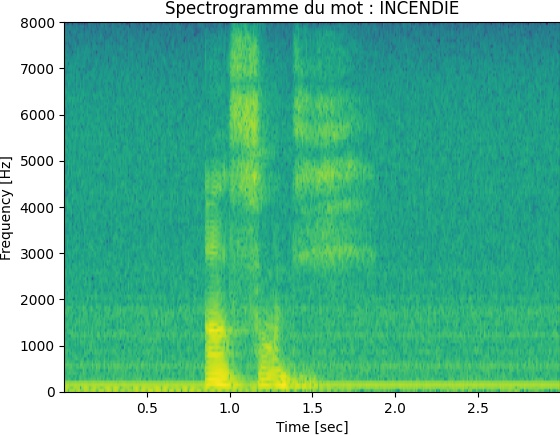
\includegraphics[width=\textwidth]{1-Incendie.jpg}
			\caption{INCENDIE}
		\end{subfigure}
		\begin{subfigure}[]{0.32\textwidth}
			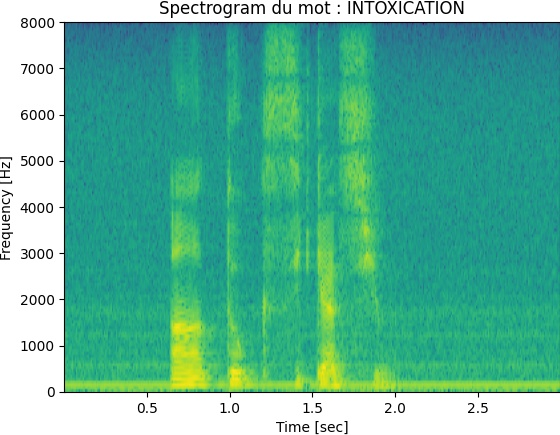
\includegraphics[width=\textwidth]{1-Intoxication.jpg}
			\caption{INTOXICATION}
		\end{subfigure}
		\begin{subfigure}[]{0.32\textwidth}
			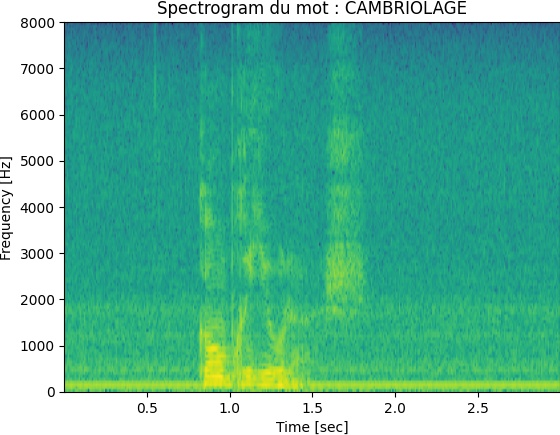
\includegraphics[width=\textwidth]{1-Cambriolage.jpg}
			\caption{CAMBRIOLAGE}
		\end{subfigure}
	\end{figure}
\end{frame}



\begin{frame}{Le découpage en formant}
	\begin{block}{Formant - Définition Larousse}
		Fréquence de résonance du conduit vocal. \\
		Les voyelles se définissent acoustiquement par leurs formants; \\
		seules les consonnes dites vocaliques présentent une structure formantique similaire à celle des voyelles.
	\end{block}
	\begin{figure}
		\begin{center}
			\centering
			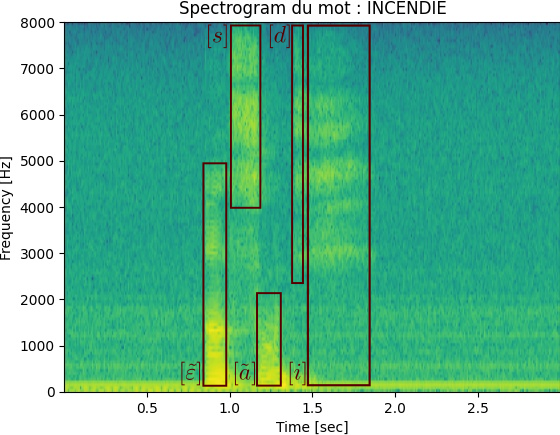
\includegraphics[width=0.45\textwidth]{3-incendie.png}
			\caption{Analyse de formant du mot "INCENDIE" \\avec l'aide de Mme.Voisin en formation d'orthophonie à la Sorbonne}
		\end{center}
	\end{figure}
\end{frame}
